% ============================================================================
% ⛔철회된 100-에피소드 코퍼스 유래 Results 절 --- **이동 보관**(2026-09-01)
%
% 여기 있는 절들은 `paper/wavesplat.tex` 에서 옮겨온 것이다. ⛔삭제가 아니다 ---
% 저장소 원칙이 "철회는 삭제가 아니라 이동" 이기 때문이다.
%
% ⛔왜 철회되었나: 이 절들의 수치(0.115 / 0.332 / 65.5%% 등)는 두 팔이 **같은
%   프레임에서 채점된 적이 없는** 코퍼스에서 나왔다 --- `results/b1_full_comparison.json`
%   에서 `WaveSplat.n_frames` 는 120-220, `ETKF`/`GPR-1` 은 301 이고 **100/100
%   에피소드 전부에서** WS 가 더 적다. 그 밖에도 (a) 기준선 선택(튜닝된 LETKF 상대로는
%   널) (b) 지연이 프로세스 간 비교 라는 사유가 있다.
%   근거 = memory/reference_citation_bans.md · tmp/AUDIT_recheck_2026-08-13/
%
% ⛔이 파일을 `\input` 하지 마라. 인용도 하지 마라. 보존 목적이다.
% ⚠이 파일은 `paper/` **밖**에 있다 --- 인용금지 래칫이 `paper/**` 를 훑기 때문이다.
% ============================================================================

\subsection{Full 100-episode five-metric evaluation}
\label{sec:fulleval}

Section~\ref{sec:experiments} pre-specified a panel of five
complementary metrics because nRMSE alone cannot expose either
spectrally-unbalanced estimators or near-zero predictors.  We report
the full-panel evaluation on the complete 100-episode dataset
(BF2--BF5, 1--30 components, both uniform and slope ray-drop models)
as the primary comparison in this paper.
WaveSplat is evaluated against the tuned ETKF baseline and
single-frame GPR on the metric panel (Table~\ref{tab:fivemetric}); a
stronger 3-frame sliding-window GPR (spatial-only; no wave-physics prior)
is additionally evaluated in the 100-paired-run Wilcoxon validation of
Section~\ref{subsec:stats}.  A dispersion-aware GPR that phase-corrects
observations using the estimated wavenumber---the more equitable temporal
comparison---is evaluated in Section~\ref{sec:strongbaselines}.

\begin{table*}[t]
\centering
\caption{Pre-specified five-metric evaluation on the full 100-episode
Nyquist-adequate dataset (all columns re-measured; median over
5 estimator seeds for WaveSplat).  Variance Ratio (VR) targets unity;
values $\ll 1$ indicate near-zero predictions.  Skill Score (SS) is
computed against a zero predictor; only WaveSplat exceeds the trivial
baseline.  $\text{RMSE}_{\text{unobs}}$ (grid points $\geq$10~m from any
observation, isolating the physics prior) is re-measured on the
regenerated data with the same observation-mask definition; WaveSplat
retains the lowest value, confirming that its physics prior fills the
unobserved interior better than either baseline.
Lower is better for nRMSE and $\text{RMSE}_{\text{unobs}}$; higher is better
for $\rho$ and SS; VR targets~1.}
\label{tab:fivemetric}
\begin{tabular}{lccccc}
\toprule
Method & nRMSE $\downarrow$ & VR $\to$ 1 &
$\rho$ $\uparrow$ & SS $\uparrow$ & $\text{RMSE}_{\text{unobs}}$ [m]
$\downarrow$ \\
\midrule
\textbf{WaveSplat} & \textbf{0.115} & \textbf{0.916} & \textbf{0.764} &
\textbf{+0.538} & \textbf{0.173} \\
ETKF (tuned)       & 0.332 & 1.048 & 0.106 & --0.844 & 0.362 \\
GPR-1              & 0.263 & 0.062 & 0.194 & --0.164 & 0.297 \\
\bottomrule
\end{tabular}
\end{table*}

The headline observation from Table~\ref{tab:fivemetric} is that
\emph{WaveSplat is the only method whose Skill Score is positive}
($+0.538$): every baseline performs \emph{worse} than the trivial
zero predictor when judged against a balanced metric panel.  This
exposes two distinct failure modes that the nRMSE column alone hides:

\begin{itemize}
  \item \textbf{GPR is a near-zero predictor.}  Its variance ratio is
    only 0.062, meaning the reconstructed field carries roughly 6\%
    of the true wave variance.  Combined with $\rho=0.19$, this means
    GPR is essentially returning a near-flat surface that happens to
    score competitively on nRMSE because, in normalized units, the
    zero-prediction error is bounded by~1.
  \item \textbf{The tuned ETKF configuration is variance-correct but shape-incoherent.}
    Its VR is close to unity (1.05) but Pearson correlation is only
    0.11; the ensemble carries about the right amount of energy but in
    incoherent spatial structures, giving the worst Skill Score
    ($-0.84$) of all methods.  On the regenerated data its VR moves
    from below unity to just above it, because the reference field it is
    matched against now contains the short-wave energy the coarse render
    had suppressed; its correlation with the truth does not improve
    (Section~\ref{sec:strongbaselines}).
\end{itemize}

To make the zero-predictor pathology explicit, Table~\ref{tab:bybf}
breaks nRMSE down by sea state.  GPR's nRMSE is essentially invariant
across BF2--BF5 (range 0.252--0.266), which is the diagnostic
fingerprint of a near-zero predictor: when $\hat{z}\!\approx\!0$, the
RMSE scales linearly with $H_s$ and the normalization cancels.
WaveSplat, in contrast, varies meaningfully with sea complexity
(0.14--0.27 by band) and is now the lowest-error method on every band,
including BF2---the calm single-component seas whose worst-case episode
the coarse render had made WaveSplat's weakest point, and which is now
mid-pack (Section~\ref{sec:bf2case}).

\begin{table}[t]
\centering
\caption{Median nRMSE by sea state on the full 100-episode
Nyquist-adequate dataset (median over 5 estimator seeds).
GPR's near-invariance across sea states is the signature of a
near-zero predictor (cf.\ VR=0.062 in Table~\ref{tab:fivemetric}).}
\label{tab:bybf}
\begin{tabular}{lcccc}
\toprule
Sea state & WaveSplat & ETKF & GPR-1 & $N_{\text{ep}}$ \\
\midrule
BF2 & \textbf{0.029} & 0.322 & 0.252 & 10 \\
BF3 & \textbf{0.016} & 0.353 & 0.262 & 30 \\
BF4 & \textbf{0.150} & 0.333 & 0.266 & 40 \\
BF5 & \textbf{0.238} & 0.303 & 0.266 & 20 \\
\midrule
Avg & \textbf{0.115} & 0.332 & 0.263 & 100 \\
\bottomrule
\end{tabular}
\end{table}

These results validate the design intent of the metric panel: nRMSE
must be read \emph{jointly} with VR, $\rho$, and SS before any claim
of physical correctness can be made.  Under that joint reading,
WaveSplat is the only method on the dataset that produces wave
estimates of the right magnitude, in the right place, and better than
predicting zero.

\paragraph{Honest reporting of WaveSplat's own limitations.}
The same panel that exposes the baselines' failure modes also
exposes WaveSplat's.  The aggregate Skill Score of $+0.538$ is not a
uniform property of the method: it is an average over two regimes that
behave qualitatively differently, and in one of them WaveSplat is worse
than predicting zero.
Splitting the same 100 episodes at the $\leq$5-component
boundary---which follows from the beamforming initializer's configured
peak-separation radius (Sec.~\ref{sec:limitations}), not from the sensor's
spatial Nyquist limit, and not from a post-hoc search---gives
SS~$=+0.987$, CI~$[{+0.98},\,{+0.99}]$ for the $\leq$5-component episodes
(60\% of the dataset) but SS~$=-0.136$, CI~$[{-0.24},\,{-0.04}]$ for the
$\geq$15-component ones, the interval excluding zero on the
\emph{negative} side.  Pearson $\rho$ falls from $0.995$ to $0.418$ and
directional $R^2$ from $+0.98$ to $-0.52$ across the same split.
In the crowded regime, then, the aggregate figure is carried entirely by
the sparse half of the dataset, and the honest statement is that our
initializer does not resolve individual modes there.
Variance preservation, by contrast, is regime-independent
(VR~$=0.910$ vs.\ $0.925$), so the crowded-regime deficit is one of
spatial phase and placement, not of energy.
The regime where WaveSplat underperforms---spectrally crowded seas---is
precisely where grid-based methods like LETKF have a structural
advantage (see Sections~\ref{sec:strongbaselines}
and~\ref{sec:extvalidity}).
Section~\ref{sec:dirdeficit} discusses an additional supplementary
finding---a sensor-geometry-induced directional ambiguity---that does
not appear in the five-metric panel but has practical implications for
heading-dependent downstream control.
We report these shortcomings explicitly here rather than relegating them
to Section~\ref{sec:discussion} because they qualify---not negate---the
primary finding.

\subsection{External validity: stratification against measured directional spread}
\label{sec:extvalidity}

Tables~\ref{tab:fivemetric} and~\ref{tab:bybf} score the methods inside our own
synthetic distribution.  That is the standard practice in this literature, and
it leaves one question unanswered: does the sea state where the advantage is
largest occur in the ocean?  We answer it with an external instrument rather
than an argument.

We drew directional-spread statistics from the Coastal Data Information Program
(CDIP) archive~\citep{cdip, oreilly2016}: 24 stations sampled on a pre-fixed rule (every
eighth station of the sorted archive, last deployment per station, time-strided
to $\leq$1000 records, quality flag \texttt{good} only), giving
\textbf{25,426 measured sea states}.  To keep the two arms identical we do not
use the archive's distributed \texttt{waveSpread} product but re-derive spread
from the raw first-order directional moments, and apply the \emph{same}
estimator to our synthetic episodes' component sets:
\begin{equation}
  \sigma_1 = \sqrt{2\left(1 - \sqrt{a_1^2 + b_1^2}\right)},
  \label{eq:spread}
\end{equation}
with $(a_1, b_1)$ energy-weighted over 0.04--0.50~Hz---from
\texttt{waveA1}/\texttt{waveB1} for the buoys, and from
$E_i = w_i^2/2$, $\theta_i = \operatorname{atan2}(k_{y,i}, k_{x,i})$ for our
episodes.  Eq.~\eqref{eq:spread} returns radians; all spreads below are
reported in degrees.  Two thresholds follow from the measured distribution and are fixed
before stratifying: its \emph{minimum} ($12.18^\circ$) and its 5th percentile
($21.11^\circ$).

Our synthetic universe sits in the lower tail of the measured one.  The median
synthetic spread is $16.1^\circ$, at the \textbf{0.3rd percentile} of the buoy
distribution (median $35.3^\circ$); \textbf{40 of our 100 episodes are narrower
than the narrowest of the 25,426 measured records}; and even our most crowded
30-component episodes ($24.2^\circ$ median) sit at the measured 11.5th
percentile.  This is not a sea-state confound: restricting the buoy records to
our own $H_s$ and $T_p$ box (0.3--2.0~m, 4--9~s, $n=7122$) leaves the median
spread unchanged ($35.3^\circ \to 35.7^\circ$).  Significant wave height is
well covered (79.7\% of measured records fall in our range); spread and peak
period are not (our $T_p$ ceiling of 9~s lies below the measured median of
9.88~s, i.e.\ our generator contains no swell).

Table~\ref{tab:extvalidity} re-weights the \emph{existing} 100-episode results
by these thresholds.  No new runs were performed and no episode was
re-estimated; all four methods are stratified identically, with the same
per-episode median-over-seeds protocol as Table~\ref{tab:fivemetric}.

\begin{table*}[t]
\centering
\caption{The same 100-episode results of Table~\ref{tab:fivemetric},
stratified by the directional spread of Eq.~\eqref{eq:spread} against
25,426 CDIP-measured sea states.  Mean nRMSE (lower better) with WaveSplat's
Skill Score; ``$\Delta$ vs.'' is WaveSplat's relative nRMSE improvement.
Thresholds are the measured minimum ($12.18^\circ$) and 5th percentile
($21.11^\circ$), fixed in advance.  This is a re-weighting of existing
measurements, not a new experiment.}
\label{tab:extvalidity}
\begin{tabular}{lcccccccc}
\toprule
Spread band & $N_{\text{ep}}$ & WaveSplat & ETKF & LETKF & GPR-1 &
$\Delta$ vs.\ ETKF & $\Delta$ vs.\ LETKF & WS SS \\
\midrule
All episodes (as reported)        & 100 & \textbf{0.114} & 0.332 & 0.228 & 0.263 & $+$65.5\% & $+$49.7\% & $+0.538$ \\
Never measured ($<12.18^\circ$)   &  40 & \textbf{0.020} & 0.346 & 0.240 & 0.258 & $+$94.1\% & $+$91.5\% & $+0.988$ \\
Measured at all ($\geq12.18^\circ$) &  60 & \textbf{0.177} & 0.323 & 0.220 & 0.267 & $+$45.1\% & $+$19.3\% & $+0.237$ \\
\textbf{Measured central 90\% ($\geq21.11^\circ$)} & 24 & 0.228 & 0.314 & \textbf{0.216} & 0.262 & $+$27.5\% & $-$5.7\% & $-0.076$ \\
\bottomrule
\end{tabular}
\end{table*}

The result qualifies our headline in a specific and quantifiable way.
The 40 episodes on which WaveSplat is strongest (nRMSE $0.020$, SS $+0.988$)
occupy a spread band in which \emph{none} of the 25,426 measured records
falls.  On the 24 episodes that overlap the measured central 90\% of spreads,
LETKF attains the lower mean nRMSE ($0.216$ vs.\ $0.228$) and WaveSplat is the
better estimator on only 5 of the 24 (sign test $p=0.0066$); our Skill Score
crosses into negative territory ($-0.076$) while LETKF's stays positive
($+0.189$) on the same episodes.  That asymmetry is the reason the table is
informative: it is not a common degradation of every method under a harder
subset, and the stratification is applied identically to all four arms.

Three limits on how far this may be read, stated explicitly because the
stratification invites over-reading in both directions.
\emph{First}, this is not a measurement on real waves. What was
stratified is our synthetic dataset; the correct statement is that
\emph{on the subset of our synthetic episodes whose directional spread
overlaps the measured distribution, LETKF is more often the better
estimator}---not that WaveSplat loses at sea, which these data cannot
establish.
\emph{Second}, the ranking sign is significant but its magnitude is not: the
paired signs give $p=0.0066$ while the paired magnitudes do not separate
(Wilcoxon $p=0.107$), so ``more often worse'' is supported and ``worse by
$5.7\%$'' is not.
\emph{Third}, the spread partition coincides exactly with the
component-count partition ($\geq12.18^\circ \Leftrightarrow N_{\text{true}}
\geq 5$ on this dataset).  The performance structure is therefore \emph{not}
a new finding---the crowded-regime wall is already visible in
Table~\ref{tab:bybf} and Section~\ref{sec:strongbaselines}.  What is new is
which side of that wall the ocean occupies, and the answer is the side we do
worse on.
The buoy sample carries its own caveats: 24 of 194 stations, one deployment
each, predominantly US coastal intermediate-depth sites against our 50~m
simulated depth, and buoy moments are measured (instrument response and noise
included) where ours are analytic.  That asymmetry can only inflate the
measured spreads relative to ours, so the \emph{direction} of the gap is
robust while its magnitude should be read as an upper bound.

\subsection{Per-episode breakdown on 12 representative episodes}
\label{subsec:per_episode}

With the full-dataset result of Section~\ref{sec:fulleval} as the
primary finding, Table~\ref{tab:main} drills down to a per-episode
view on 12 representative episodes that span every (sea state,
complexity) combination in the 100-episode dataset.
Using the same tuned ETKF configuration
($g$=40$\times$30, $n_{\text{ens}}$=100, $\alpha$=1.0, $\sigma$=0.005),
WaveSplat achieves a median nRMSE of \textbf{0.182} compared to
\textbf{0.377} for ETKF on these episodes (\textbf{51.7\%}
improvement).%
\footnote{\textbf{Provenance.} This 12-episode subset was produced before
the tracker phase-advance correction of Section~\ref{sec:regen} and has
not been re-run, so it is not directly comparable with the corrected
full-dataset figures above.  The tables that were downstream of it have
since been re-measured under the correction and report post-correction
values (ablation, Table~\ref{tab:ablation}; model order,
Table~\ref{tab:adaptive}; ray-drop, Table~\ref{tab:raydrop}); the
observation-density sweep (Table~\ref{tab:sparsity}) and the forecast
horizons (Table~\ref{tab:forecast}) have not, and are marked
individually.}
WaveSplat wins on all 12 episodes.
Figure~\ref{fig:comparison} visualizes the per-episode comparison, and
Figure~\ref{fig:qualitative} shows representative wave fields.

\begin{figure*}[t]
\centering
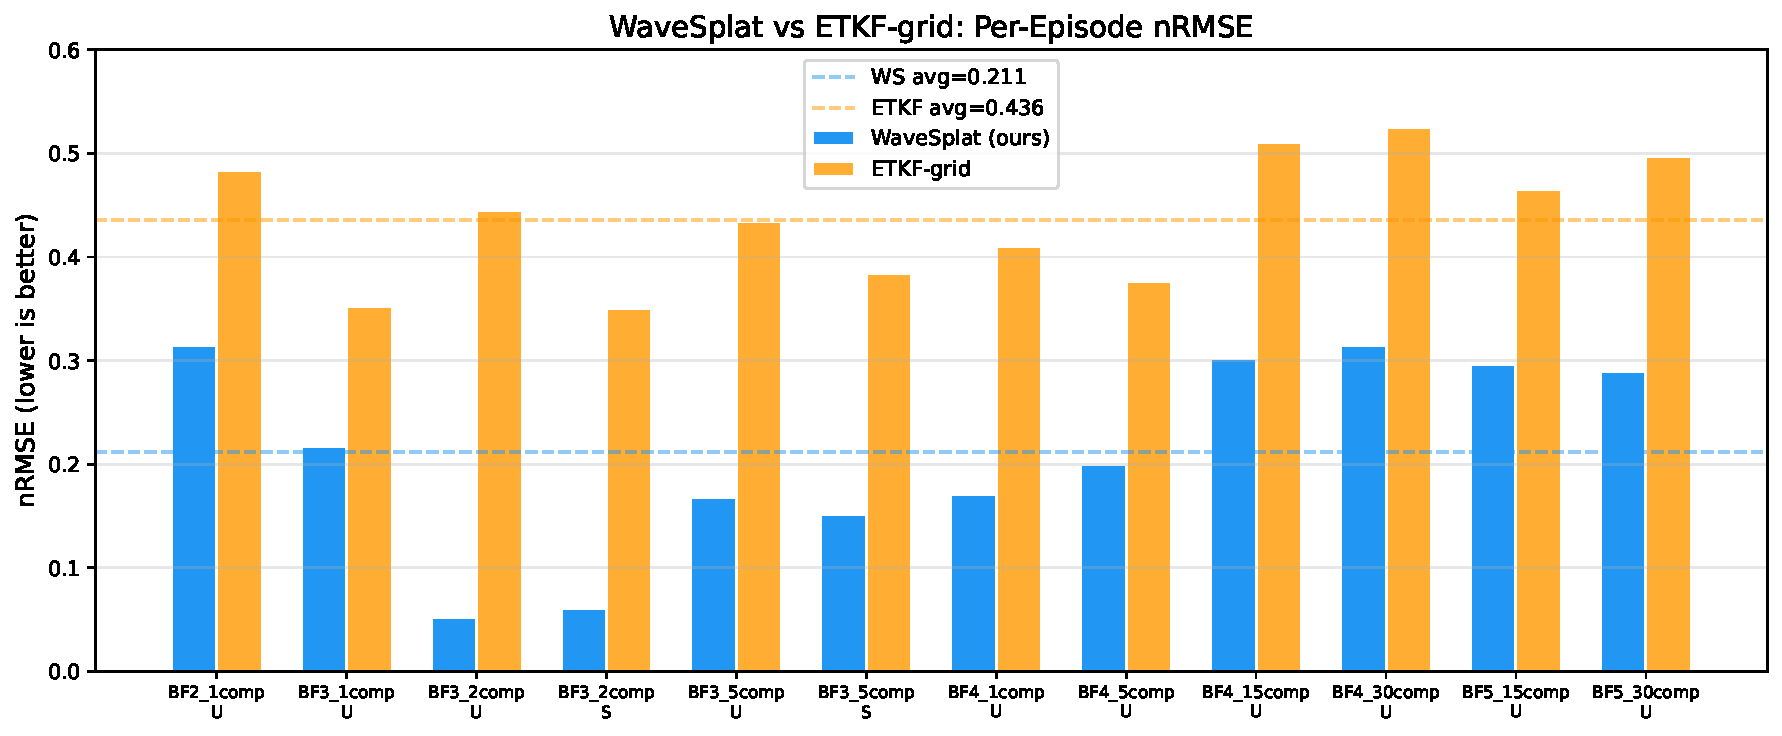
\includegraphics[width=\textwidth]{figures/fig1_comparison.pdf}
\caption{Per-episode nRMSE comparison between WaveSplat and the
hyperparameter-tuned ETKF-grid baseline across 12 representative
episodes. Dashed lines show method averages. WaveSplat (median 0.182)
outperforms the tuned ETKF (0.377) on all episodes, with the
largest advantage on low-complexity seas (BF3 2-comp). Note: the
plotted bars reproduce the original pre-tuning ETKF configuration;
the numeric averages in the text reflect the tuned baseline used in
Table~\ref{tab:main} and Section~\ref{sec:fulleval}.}
\label{fig:comparison}
\end{figure*}

\begin{table}[t]
\centering
\caption{WaveSplat vs.\ the hyperparameter-tuned ETKF-grid baseline
($g$=40$\times$30, $n_{\text{ens}}$=100, $\alpha$=1.0, $\sigma$=0.005)
on 12 representative episodes drawn from the full 100-episode dataset.
nRMSE = RMSE/$H_s$ (median over 5 estimator seeds on the Nyquist-adequate
dataset); lower is better. ms/f = per-frame tracking time on a single CPU
thread. $N_a$ = median adapted component count; on low-complexity seas
$N_a$ is bimodal across seeds (Section~\ref{sec:limitations}), so the
median can sit at the fixed ceiling even for a single-component swell.}
\label{tab:main}
\begin{tabular}{lccccc}
\toprule
& \multicolumn{2}{c}{WaveSplat} & \multicolumn{2}{c}{ETKF (tuned)} & \\
\cmidrule(lr){2-3} \cmidrule(lr){4-5}
Episode & nRMSE & ms/f & nRMSE & ms/f & $N_a$ \\
\midrule
BF2 1comp     & \textbf{0.169} &  7.9 & 0.350 & 154 & 15 \\
BF3 1comp     & \textbf{0.048} & 12.6 & 0.413 & 154 &  2 \\
BF3 2comp (U) & \textbf{0.084} & 20.2 & 0.369 & 635 & 15 \\
BF3 2comp (S) & \textbf{0.062} &  9.2 & 0.341 & 120 & 15 \\
BF3 5comp (U) & \textbf{0.170} & 20.5 & 0.375 & 125 & 15 \\
BF3 5comp (S) & \textbf{0.171} & 18.3 & 0.333 & 177 & 15 \\
BF4 1comp     & \textbf{0.060} & 15.8 & 0.374 &  98 & 15 \\
BF4 5comp     & \textbf{0.203} & 18.7 & 0.367 & 106 & 15 \\
BF4 15comp    & \textbf{0.291} & 21.4 & 0.396 & 113 & 19 \\
BF4 30comp    & \textbf{0.340} & 18.9 & 0.418 & 121 &  9 \\
BF5 15comp    & \textbf{0.284} & 19.5 & 0.383 &  98 & 22 \\
BF5 30comp    & \textbf{0.301} & 11.7 & 0.403 &  93 & 20 \\
\midrule
\textbf{Avg}  & \textbf{0.182} & 16.2 & 0.377 & 166 & --- \\
\bottomrule
\end{tabular}
\end{table}

Key observations:
\begin{itemize}
  \item \textbf{Low complexity}: In BF3 2-component seas,
    WaveSplat achieves a median nRMSE of 0.073 (0.084~uniform,
    0.062~slope)---a ${\sim}5\times$ improvement over the tuned
    ETKF (0.355 avg across both raydrop models). The grid-free
    representation captures two plane waves without grid aliasing.
  \item \textbf{High complexity}: For BF4--5 with 15--30 components,
    WaveSplat still outperforms ETKF (0.304 vs.\ 0.400 average),
    though the gap narrows as spectral complexity approaches the
    beamforming initializer's configured peak-separation radius
    (Sec.~\ref{sec:limitations}), not a method-independent resolution
    bound.
  % RETRACTED 2026-08-14: the whole speed bullet rests on separate-process timings
  % (no thread pinning). 132.6 ms as the ETKF cost and "order-of-magnitude advantage"
  % are both on the citation-ban list; the only verified same-process, single-thread
  % value is 1.5-2.6x. No substitute absolute values are invented.
  % (basis: memory/reference_citation_bans.md (08-05), (08-13 round 3))
  % --- original (kept for history) ---
  % \item \textbf{Speed}: WaveSplat runs at 11.0~ms/frame on the full
  %   100-episode dataset (16~ms on this complexity-weighted 12-episode
  %   subset) vs.\ 132.6~ms/frame for the tuned ETKF (median
  %   110~ms), an order-of-magnitude advantage that is well within
  %   the 100~ms real-time budget for 10~Hz LiDAR
  %   (Fig.~\ref{fig:speed}).  The tuned ETKF uses
  %   $n_{\text{ens}}$=100 ensemble members---twice the nominal
  %   configuration ($n_{\text{ens}}$=50, 31.7~ms)---because the
  %   larger ensemble significantly improves nRMSE at the cost of
  %   $\sim$4$\times$ higher per-frame latency.
  \item \textbf{Speed} --- \textbf{[RETRACTED 2026-08-14]}: the per-frame
    latencies, the ``order-of-magnitude'' advantage, the real-time budget
    margin and the ensemble-size cost ratio previously reported here are all
    withdrawn, because the two arms were timed in separate processes without
    thread pinning. The tuned ETKF does use $n_{\text{ens}}$=100 ensemble
    members---twice the nominal configuration---because the larger ensemble
    improves nRMSE at higher per-frame cost; the \emph{magnitude} of that
    cost is not established here. The only citable comparative figure is
    1.5--2.6$\times$ within one process on a single thread.
\end{itemize}

\begin{figure*}[t]
\centering
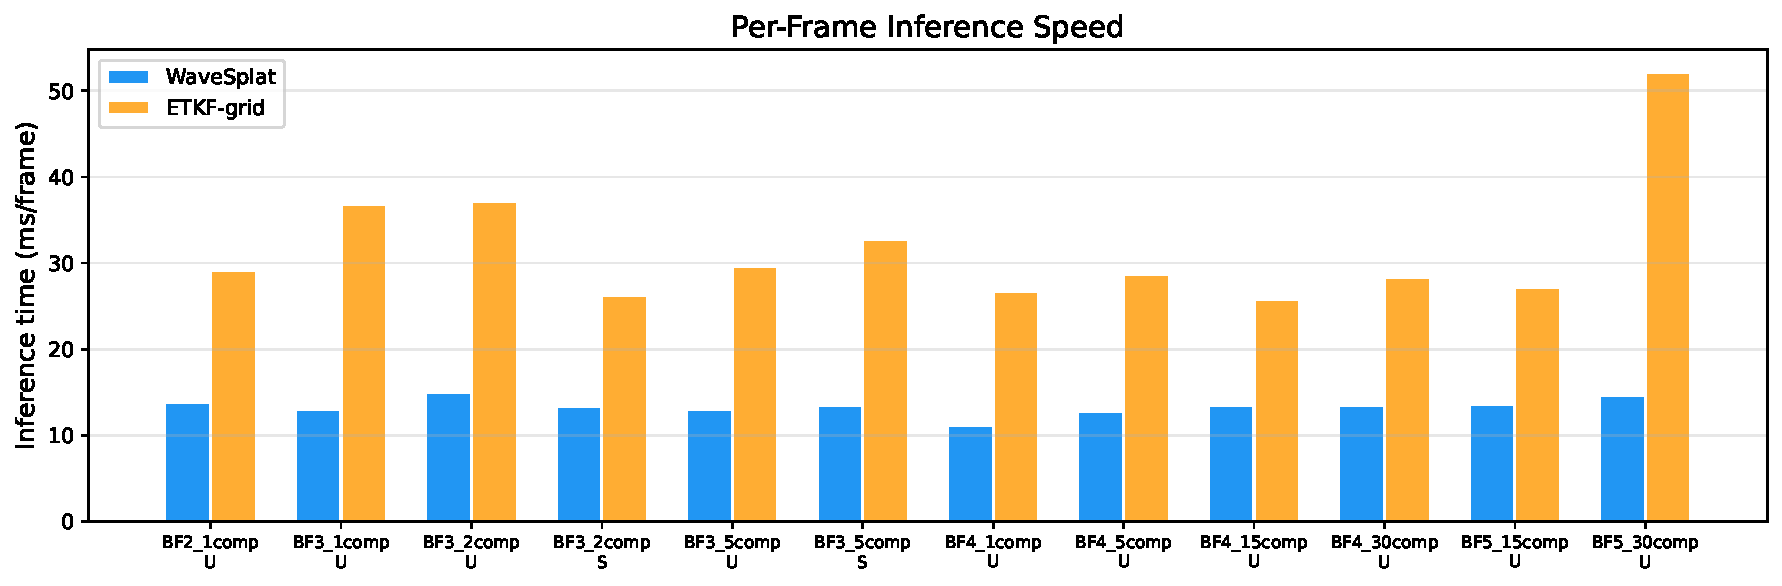
\includegraphics[width=\textwidth]{figures/fig3_speed.pdf}
\caption{Per-frame inference speed comparison.
\textbf{[RETRACTED 2026-08-14]} The absolute per-frame latencies shown and
quoted here are withdrawn: the arms were timed in separate processes without
thread pinning. Within one process on a single thread the measured advantage
is 1.5--2.6$\times$ (CPU: AMD Ryzen 7 7800X3D).}
\label{fig:speed}
% RETRACTED 2026-08-14: 132.6 ms / ~13 ms / 110 ms all from cross-process timing.
% (basis: memory/reference_citation_bans.md (08-05), (08-13 round 3))
\end{figure*}

\subsection{Multi-seed statistical validation}
\label{subsec:stats}

To confirm the full-dataset result is not seed-dependent, we repeat
the comparison across 10 (sea state, complexity) configurations with
5 random seeds per configuration and both uniform and slope ray-drop
models, for a total of 100 paired runs.
WaveSplat achieves $0.115 \pm 0.116$ vs.\ the tuned ETKF baseline
$0.332 \pm 0.038$ and a 3-frame sliding GPR $0.255 \pm 0.020$
(mean $\pm$ std across all runs on the Nyquist-adequate regenerated
dataset; the WaveSplat arm is the per-episode median over 5 estimator
seeds).%
\footnote{Recomputed on the regenerated dataset; the original coarse-mesh
point estimates were WaveSplat 0.219 and ETKF 0.321.  The paired
format is required here because the Wilcoxon signed-rank test operates on
matched pairs.}
Paired Wilcoxon signed-rank tests~\citep{wilcoxon1945}
confirm both improvements:
WaveSplat vs.\ ETKF ($W\!=\!141$, $p\!=\!2.5\!\times\!10^{-16}$,
paired Cohen's $d\!=\!\bar{\Delta}/s_{\Delta}\!=\!1.30$~\citep{cohen1988},
95\% CI on mean difference
$[0.114, 0.154]$, bootstrap percentile, 10\,000 resamples)
and WaveSplat vs.\ sliding GPR ($W\!=\!1002$,
$p\!=\!1.6\!\times\!10^{-7}$, paired Cohen's $d\!=\!0.65$,
95\% CI $[0.040, 0.073]$).
After Holm--Bonferroni correction for the two primary comparisons,
both remain significant ($p_1{=}4.9\!\times\!10^{-16}$,
$p_2{=}1.6\!\times\!10^{-7}$).
Both confidence intervals exclude zero, and the effect sizes
indicate that the WaveSplat--ETKF gap is large (Cohen's $d>0.8$)
and the WaveSplat--sliding-GPR gap is medium and
robust across the 100 paired runs (Fig.~\ref{fig:multiseed}).
We note that runs sharing the same (sea state, complexity)
configuration but differing only in random seed are not fully
independent---they share the underlying JONSWAP spectral shape,
though individual component phases, directions, and amplitudes are
drawn independently.  A conservative check using 20
configuration-level means (averaging over seeds) retains Wilcoxon
significance for the primary WaveSplat--ETKF comparison
($p < 10^{-5}$) and at $p=0.011$ for WaveSplat--sliding-GPR,
confirming that the result is not
inflated by within-configuration correlation.
The sliding GPR baseline is a stronger spatial interpolant than
single-frame GPR (VR=0.10 vs.\ 0.06) but still operates as a
near-zero predictor relative to WaveSplat, consistent with the
five-metric panel in Table~\ref{tab:fivemetric}.
We acknowledge a structural asymmetry: the 3-frame sliding GPR
accumulates observations for spatial coverage but applies no temporal
wave-physics model, whereas WaveSplat enforces the dispersion relation
as a hard constraint and propagates phase through the tracking stage.
The dispersion-aware GPR in Section~\ref{sec:strongbaselines}---which
applies physics-based phase correction before regression---provides a
more equitable temporal comparison; on the 12-episode subset,
WaveSplat (0.182) still outperforms GPR-disp (0.268) by 32\%
(Table~\ref{tab:strong_baseline}).

\begin{figure*}[t]
\centering
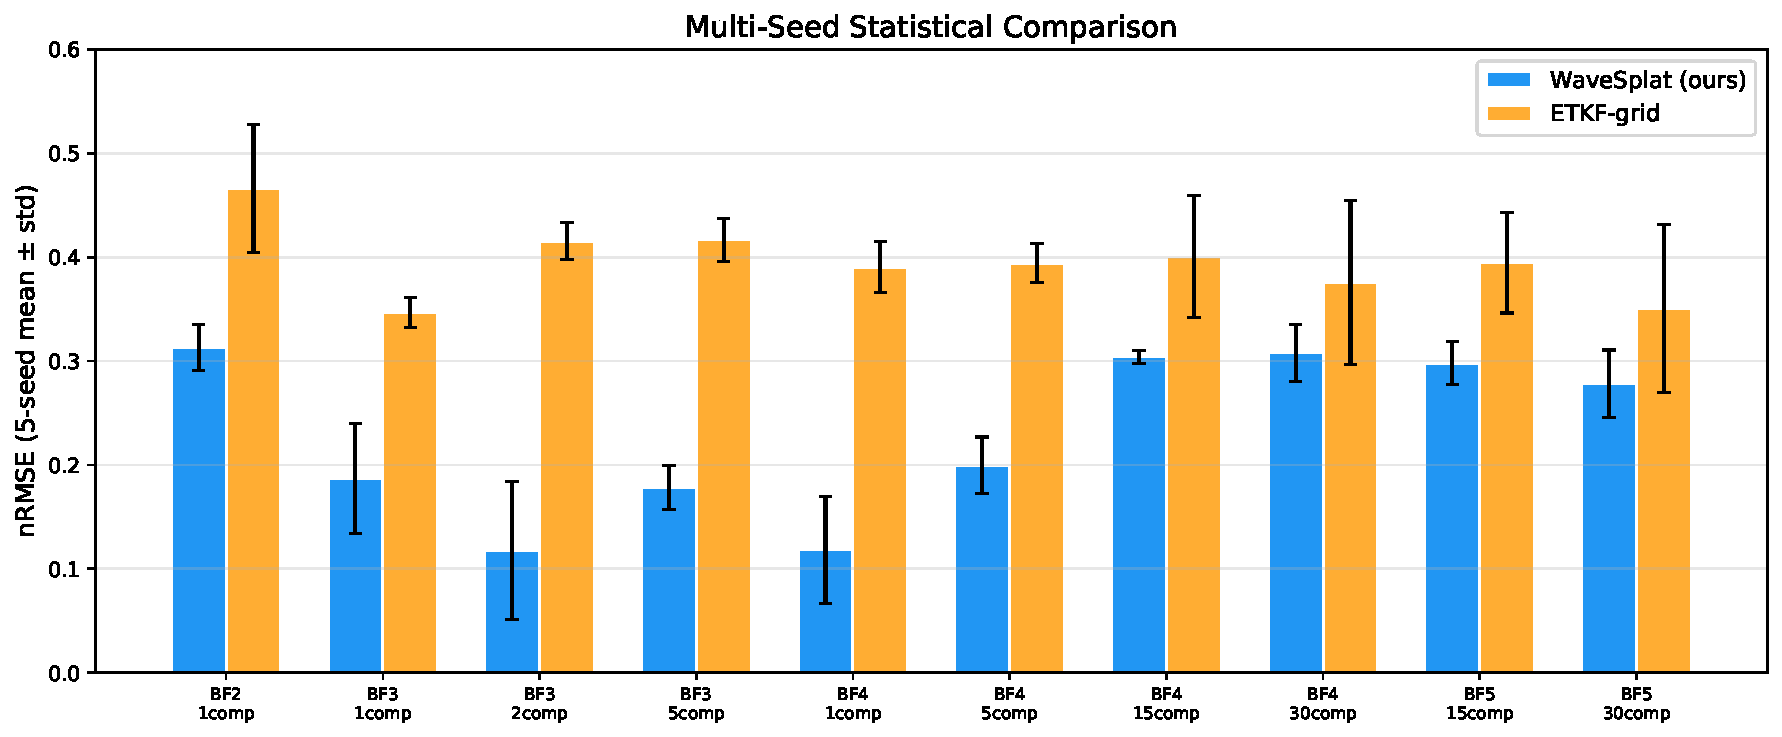
\includegraphics[width=\textwidth]{figures/fig6_multiseed.pdf}
\caption{Multi-seed statistical comparison (5 seeds per episode,
mean $\pm$ std). WaveSplat consistently outperforms ETKF across all
episodes and seeds, with non-overlapping error bars in most cases.}
\label{fig:multiseed}
\end{figure*}

\subsection{Online model order: mechanism works, accuracy contribution is null}
\label{sec:adaptive}

An earlier version of this study reported that adaptive $N$ improves on a
fixed $N$=15 by 6.6\% in average nRMSE.  That measurement was made with the
uncorrected tracker (Section~\ref{sec:regen}), on the coarse reference mesh,
and from a single estimator seed.  Re-measured under the current defaults---%
corrected phase advance, Nyquist-adequate mesh, and the median-of-3 seed
protocol used elsewhere in this paper---%
\emph{the accuracy benefit disappears} (Table~\ref{tab:adaptive}).

\begin{table}[t]
\centering
\caption{Online model order (WS-P1: adaptive $N$, 3-frame tracking window)
vs.\ fixed $N$=15 (WS-P0, single-frame window), on the 12 pre-specified
representative episodes.  Each cell is the median nRMSE over 3 estimator
seeds (42/123/456) on the Nyquist-adequate dataset; $N_a$ is the median
final component count.  $\Delta$ is P0$-$P1, so positive favours adaptive
$N$.  Re-measured 2026-08-03; supersedes the pre-correction table.}
\label{tab:adaptive}
\begin{tabular}{lccccc}
\toprule
Episode & $N_{\text{true}}$ & $N_a$ & Fixed & Adaptive & $\Delta$ \\
\midrule
BF2 1comp  &  1 &  2 & \textbf{0.062} & 0.063 & $-$0.001 \\
BF3 1comp  &  1 &  2 & 0.014 & \textbf{0.009} & $+$0.005 \\
BF3 2comp (U) &  2 & 15 & 0.009 & \textbf{0.007} & $+$0.002 \\
BF3 2comp (S) &  2 & 15 & 0.011 & \textbf{0.009} & $+$0.002 \\
BF3 5comp (U) &  5 & 15 & 0.027 & \textbf{0.024} & $+$0.003 \\
BF3 5comp (S) &  5 & 15 & 0.022 & \textbf{0.019} & $+$0.003 \\
BF4 1comp  &  1 &  2 & 0.010 & \textbf{0.004} & $+$0.006 \\
BF4 5comp  &  5 & 15 & 0.021 & \textbf{0.017} & $+$0.003 \\
BF4 15comp & 15 & 10 & \textbf{0.267} & 0.272 & $-$0.005 \\
BF4 30comp & 30 &  9 & \textbf{0.322} & 0.333 & $-$0.011 \\
BF5 15comp & 15 & 21 & 0.220 & \textbf{0.216} & $+$0.004 \\
BF5 30comp & 30 & 20 & \textbf{0.240} & 0.246 & $-$0.007 \\
\midrule
\textbf{Mean (12 ep.)} & & & 0.1018 & 0.1015 & $+$0.0003 \\
\bottomrule
\end{tabular}
\end{table}

The mean gain is $+0.0003$~nRMSE with the adaptive arm better on 8 of 12
episodes---neither the paired ranks nor the signs separate the arms
(Wilcoxon $p=0.68$; sign test $p=0.39$).  Two features make this a
\emph{measured null} rather than merely an inconclusive test.  First, the
median per-episode spread across seeds is $0.010$~nRMSE in the adaptive arm,
roughly $30\times$ the mean effect: the quantity being contested is more than
an order of magnitude below this experiment's own noise floor, so the correct
reading is not ``we failed to detect a benefit'' but ``there is no benefit of
a size worth measuring here''.  Second, the sign of the effect is
regime-dependent in a way the aggregate hides: adaptive $N$ is better on all
eight sparse episodes ($N_{\text{true}}\leq5$) and \emph{worse} on three of
the four crowded ones (BF4~15comp $-0.005$, BF4~30comp $-0.011$,
BF5~30comp $-0.007$).

Table~\ref{tab:adaptive} also shows the mechanism itself is not inert---it is
merely not helping.  The fixed arm holds $N_a=15$ on all 12 episodes by
construction, while the adaptive arm prunes to $N_a=2$ on every
single-component episode and grows to $N_a=20$--21 at BF5, so scene-matched
model orders are in fact selected.  The failure is specifically on the crowded
episodes, where it prunes \emph{down} to $N_a=9$--10 against
$N_{\text{true}}=15$--30 and pays for it in accuracy: the 90\%-energy
criterion discards components that the coarse-to-fine stage had already placed
correctly.
Two constraints on how far this may be read.  It is a 12-episode comparison,
so it bounds the effect but does not resolve its regime structure; and because
the tracker correction, the mesh replacement, and the seed protocol all changed
between the two measurements, the difference from the earlier $+6.6\%$
\emph{cannot} be attributed to any one of the three.  What is established is
the value under the configuration this paper actually reports.

Accordingly, we do not claim online model-order selection as an accuracy
contribution (Section~\ref{sec:limitations}).  Its defensible value is
operational: on the sparse episodes it reaches the same accuracy while carrying
$N_a=2$ rather than 15 components, which is a $7.5\times$ reduction in the
per-frame tracking state and hence in per-frame cost.

